%%===========================================================%%
%%                                                           %%
%%                          DATASET                          %%
%%                                                           %%
%%===========================================================%%


\chapter{Data set}\label{chap:dataset}

\section{Trigger}\label{seq:trigger}

The main trigger designed for studies of Central Diffraction in run 15 was RP\_CPT2. It was formed of the following conditions combined by logical AND (\&\&):
\begin{enumerate}
 \item \textbf{(ET \&\& !IT) $||$ (!ET \&\& IT)} = signal in at least one RP on each side of the STAR central detector - to ensure presence of two forward-scattered protons; a veto was imposed on simultaneous signal in RPs above and below the beamline, which might have originated either from proton dissociation, or pile-up event, or beam halo proton etc.,
 \item \textbf{!BBCE \&\& !BBCW \&\& !ZDCE \&\& !ZDCW} = veto on any signal in small BBC tiles or ZDCs on any side of STAR central detector - such requirement is in accordance with the double-gap topology of CEP events, it mostly filtered out CEP events with parallel pile-up event(s),
 \item \textbf{TOF$\geq$2} = at least 2 hits in TOF - aim of this condition was to ensure activity in the mid-rapidity; since the lowest multiplicity allowed in CEP is 2, that was the lower threshold of L0 TOF multiplicity.
\end{enumerate}%
This trigger was running with an average prescale of 5 and average DAQ rate of 250~Hz, which allowed to collect in total about 560~M events corresponding to 16.5~pb$^{-1}$ of integrated luminosity.  More information about number of events per run, rates etc. can be found under link provided in Ref.~\cite{onlineRpTriggersMonitoring}, which contains selected data from STAR run log~\cite{RunLog}. Luminosity data used in this analysis comes from Ref.~\cite{Luminosity}.

All RP triggers which were intended for usage in diffractive physics analyses or efficiency studies are listed in Tab.~\ref{tab:triggers}. Components used in definitions of these triggers are outlined in Fig.~\ref{fig:triggerBits}. Detailed explanation of all trigger bits can be found in Refs.~\cite{RpTriggers,RpTriggers2}. Explanation of naming convention in Roman Pot system can be found in Ref.~\cite{Labeling}.

\begin{figure}[h]
 \centering%
 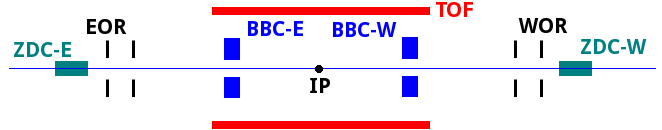
\includegraphics[width=0.71\linewidth]{graphics/dataset/bits.png}%
 \caption{Sketch of the trigger components used in definitions of diffractive triggers in run 15.}\label{fig:triggerBits}%
 \end{figure}


\begin{table}[hb!]\centering
 \begin{tabular}{l|c|c|c}%\hline
 \textbf{\specialcell{Trigger\\name}} &  \textbf{Definition} &  \textbf{\specialcell{Events [M]\\(available)}} &  \textbf{Comment} \\ \hline
 RP\_CP & {EOR \&\& WOR} & 73.3 (46.0) & \specialcell{Loose trigger (mostly elastic events) designed\\for monitoring/trigger efficiency study}\\ \hline
 RP\_CPT & {\specialcell{\specialcell{EOR \&\& WOR\\ \&\& !BBCE \&\& !BBCW} \\ \specialcell{\&\& !ZDCE \&\& !ZDCW} \\ \&\& TOF$\geq$1}} & 38.9 (0.0) & \specialcell{Intended to be main CEP trigger (later\\switched to RP\_CPT2 due to large prescale)}\\ \hline
 RP\_CPT2 & {\specialcell{\specialcell{(ET \&\& !IT) $||$ (!ET \&\& IT) \\ \&\& !BBCE \&\& !BBCW} \\ \specialcell{\&\& !ZDCE \&\& !ZDCW} \\ \&\& TOF$\geq$2}} & 556.5 (493.8) & \specialcell{Main CEP trigger\\Note: On Apr 14 added upper TOF limit (10)} \\ \hline
 RP\_CPX & {\specialcell{\specialcell{IT\\ \&\& !BBCE \&\& !BBCW} \\ \specialcell{\&\& !ZDCE \&\& !ZDCW} \\ \&\& TOF$\geq$2}} & 40.1 (0.0) & \specialcell{The same as RP\_CPT2\\but only IT configuration}\\ \hline
 RP\_CPEI & {\specialcell{\specialcell{ET \&\& IT\\ \&\& !BBCE \&\& !BBCW} \\ \specialcell{\&\& !ZDCE \&\& !ZDCW} \\ \&\& TOF$\geq$2}} & 15.6 (11.8) & \specialcell{Control trigger for CPT2 to estimate\\ effect of !(ET \&\& IT) veto } %\\ \hline
\end{tabular}\caption{Central Diffraction physics triggers and control triggers involving Roman Pot detectors in run 15.}\label{tab:triggers}
\end{table}


\section{Reconstruction software}\label{sec:recoSoftware}

Raw data was processed with STAR libraries in versions SL15f. All four trigger datasets were processed: production\_pp200trans\_2015, production\_pp200long2\_2015, production\_pp200long3\_2015 and production\_pp200long\_2015 (see~\cite{ProductionList}).

The following BFC options were used in the reconstruction:\vspace{-5pt}
\begin{verbatim}
DbV20160418,pp2015c,btof,mtd,mtdCalib,pp2pp,-beamline,beamline3D,useBTOFmatchOnly,VFStoreX,
fmsDat,fmsPoint,fpsDat,BEmcChkStat,-evout,CorrX,OSpaceZ2,OGridLeak3D,-hitfilt
\end{verbatim}
Main attention should be put on option \textbf{useBTOFmatchOnly} which forced vertexing algorithm to form vertices only from the global TPC tracks which are matched with hits in the TOF system. This solution was found to yield significantly larger signal reconstruction efficiency (vertexing efficiency) and better resolutions. The study which lead to above conclusions, presented in Ref.~\cite{RevertexingProposal}, was performed on the same dataset processed with older libraries SL15k (without useBTOFmatchOnly option).



\section{Data format}\label{sec:dataFormat}

The analyzed data was stored in ROOT files in the picoDST format which was in large part a skimmed MuDST (standard STAR format). The picoDST format was introduced in Ref.~\cite{PicoDstDescription}. PicoDST description files (C++ headers etc.) can be found in the analysis code repository~\cite{AnalysisCodeRepo}.

\section{Bad runs}\label{sec:badRuns}

Analysis of CEP was performed on the data from runs with completion status ``Successful'' in the STAR run log. However, based on additional requirements explained below, some runs were omitted from analysis.

\subsection{RP distance from the beamline}

16065025
16065026
16065027
16065028
16072057
16072058
16077055
16083006
16083007
16106031

%---------------------------
\begin{figure}[hb]
\centering
\parbox{0.4\textwidth}{
  \centering
  \begin{subfigure}[b]{\linewidth}{
                \subcaptionbox{\label{fig:positionHistograms}}{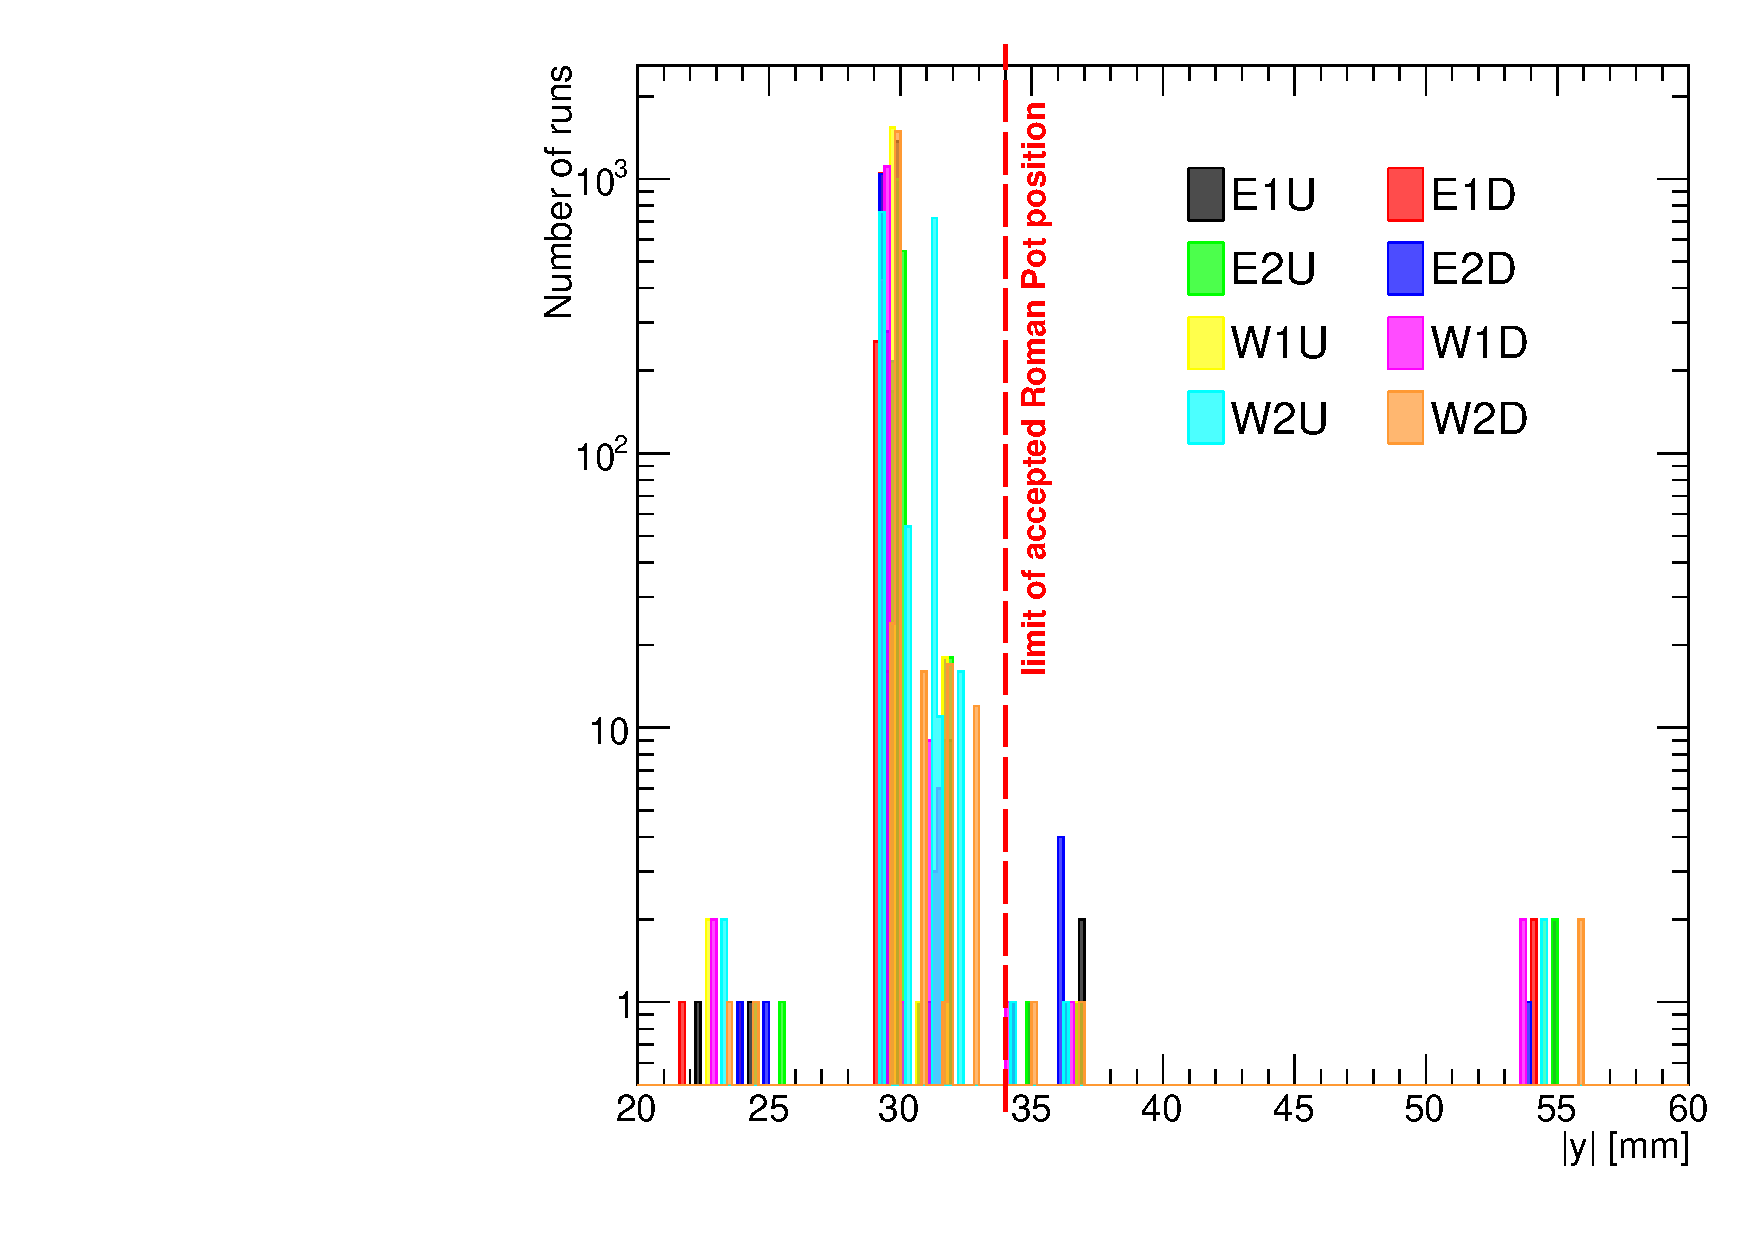
\includegraphics[width=\linewidth]{graphics/dataset/positionHistograms.pdf}}}
  \end{subfigure}
}
\quad
\parbox{0.545\textwidth}{
  \centering
  \begin{subfigure}[b]{\linewidth}{
                \subcaptionbox{\label{fig:positionVsRunGraph}}{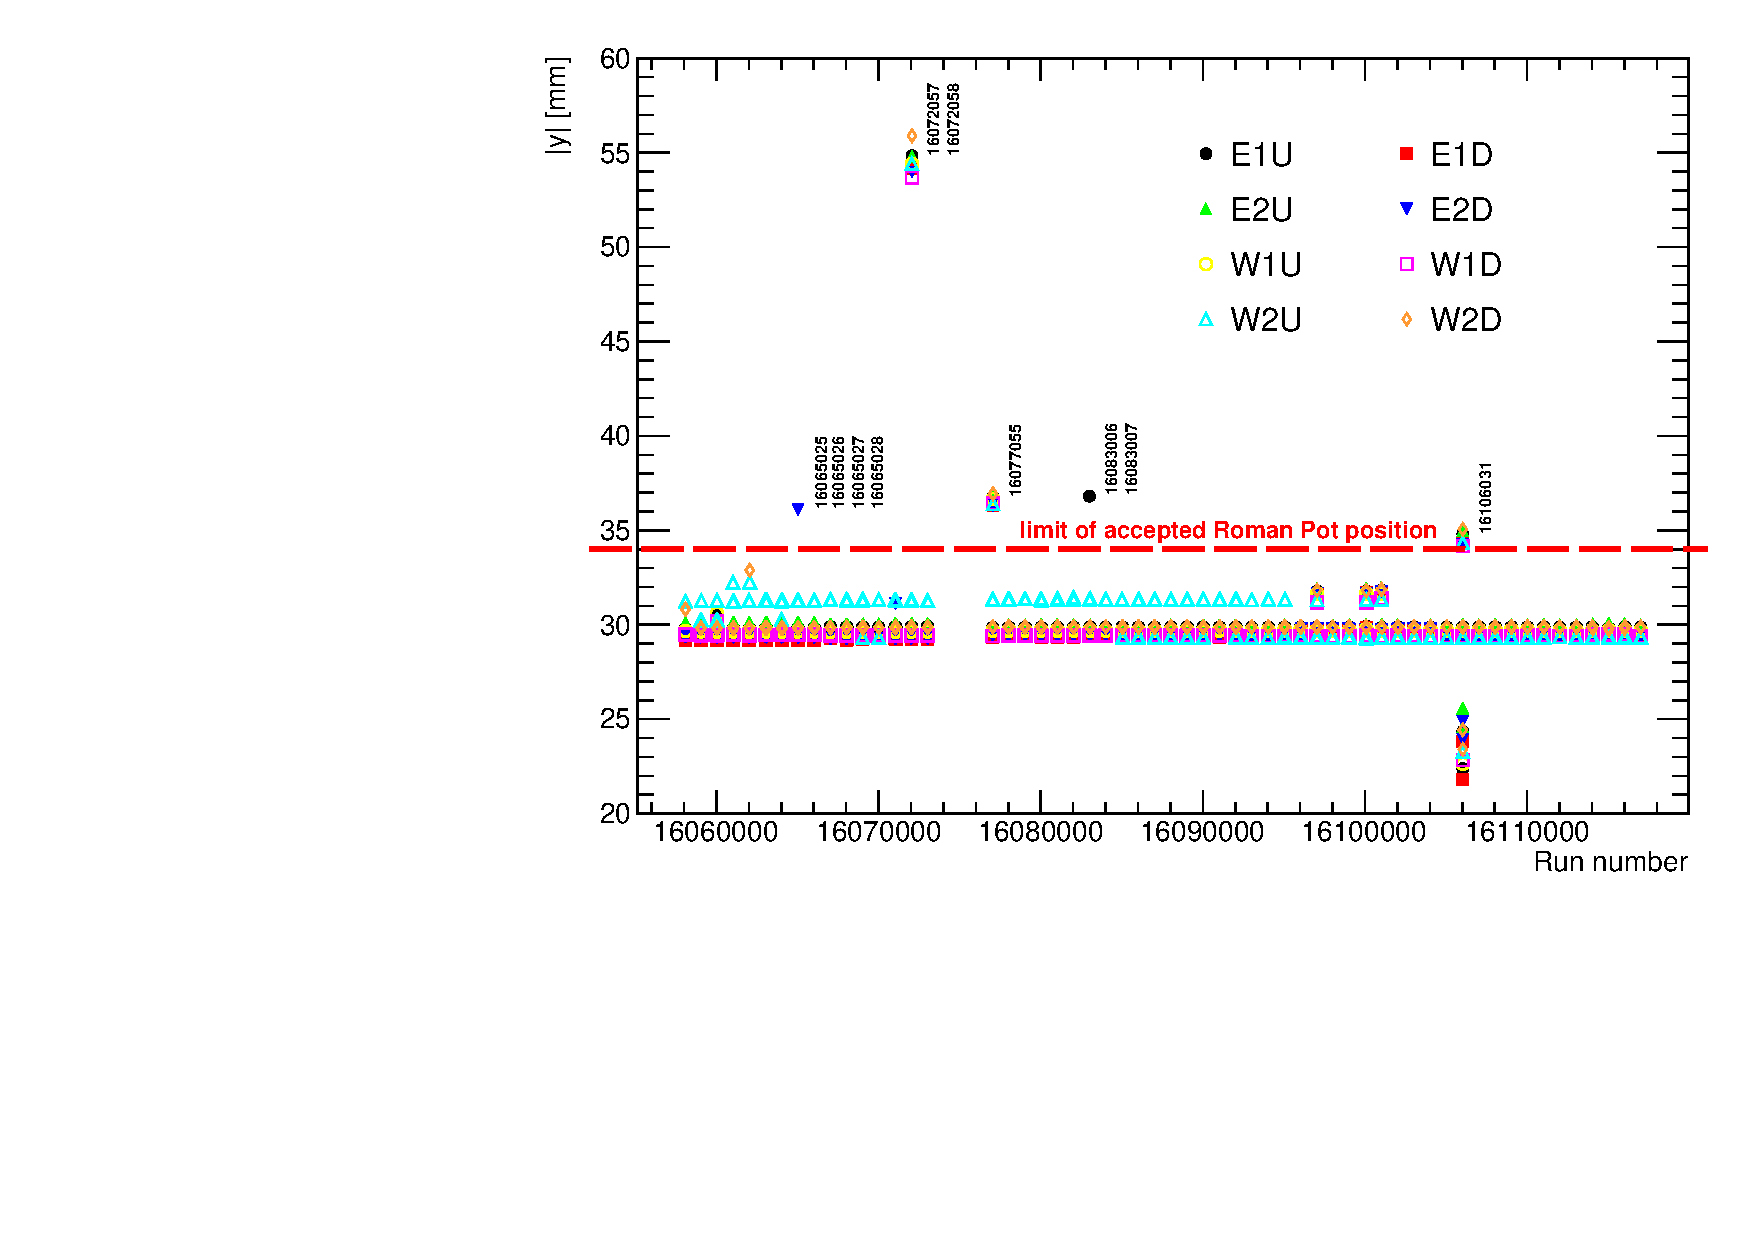
\includegraphics[width=\linewidth]{graphics/dataset/positionVsRunGraph.pdf}}}
  \end{subfigure}
}%
\caption[Beam-detector distance of the Roman Pots in run 15.]{Histogram of beam-detector distance $|y|$ (\ref{fig:positionHistograms}) and graph showing run-dependence of $|y|$ (\ref{fig:positionVsRunGraph}) for all Roman Pots.}%\label{fig:xy_recoEff}
\end{figure}
%---------------------------
